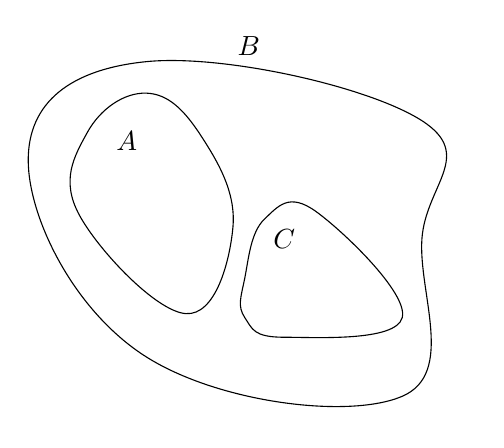
\begin{tikzpicture}[scale=0.5]
\draw[ ]  plot[smooth cycle, tension=.7] coordinates {(-9.5,4.7) (-9.7,2.6) (-7,0.1) (-5.8,2.3) (-6.6,4.6) (-8,5.7) };
\draw[ ]  plot[smooth cycle, tension=.7] coordinates { (-5,2.5) (-5.5,1) (-5.5,0) (-4.5,-0.5) (-1.5,0)   (-3.7,2.7)};

\coordinate (C) at (-5.4,6.4) {} {} {} {};
\node[above] at (C) {$ B$};
\coordinate (A) at (-8.5,4) {} {} {} {} {};
\node[above] at (A) {$A$};
\coordinate (B) at (-4.5,1.5) {} {} {} {} {};
\node[above] at (B) {$C$};
\draw  plot[smooth cycle, tension=.7] coordinates {(-11,4) (-8,-1) (-1.5,-2) (-1,2) (-1,5) (-8,6.5) };
\end{tikzpicture}